%!TEX root = ../main.tex

\centerline{\textbf{\xiaoer{开题报告}}}
\bigskip

\chapter{问题提出的背景}
\section{背景介绍}
在互联网飞速发展的今天,如何在海量数据中找到对自己真正有用的信息,越来越成为人们不得不去思考的一个问题。而推荐系统则可以为用户过滤掉低相关的内容,根据用户的兴趣、偏好,将符合用户品味的信息筛选出来,并以个性化列表的方式推荐给用户。如今,推荐系统正在不知不觉间改变着我们的生活:从社交网络(Facebook、Twitter、腾讯等)到电子商务(如Amazon、eBay、Netflix、淘宝等),从新闻推荐(如Google News、Grouplens、今日头条等)到信息检索(如iGoogle、MyYahoo、百度等)再到位置服务(如Foursquare、Yelp、大众点评等),我们无时无刻不在享受着推荐系统所带给我们的便捷。

而同时,近些年来,深度学习在图像处理,自然语言处理和语音识别等领域都取得了突破性的发展,而这也为推荐系统的进一步发展带来了新的机遇和挑战。作为推荐系统领域的顶级会议,ACM推荐系统年会(ACM RecSys)就在2016年专门召开了第一届基于深度学习的推荐系统研究专题研讨会(DLRS'16)。而研究基于深度学习的推荐系统的文章,近些年在数据挖掘和机器学习顶级会议(SIGKDD,NIPS,SIGIR,WWW,AAAI)上的发表量也是连年增加。

由此可见,利用深度学习来改进现有的推荐算法,不仅会是学术界接下来的一个研究热点,其对于传统算法的提升也会进一步方便人类生活的方方面面。
\section{推荐算法的研究现状}

传统的推荐算法主要基于两种方法或它们的组合:基于内容的方法和基于协同过滤的方法。

基于内容的推荐算法的关键在于内容的挖掘,最简单的,比如说我们从一篇新闻的正文和标题中分析出一个人名,而在评论中也分析出其他用户在讨论时也提到了这些人名,那么我们就可以进行推荐。基于内容的推荐天然优势在于推荐的可解释性强以及适合缺少用户行为的新物品的推荐。但这种方法依赖于有效的特征提取,例如,在视频推荐中\cite{Sarwar01item-basedcollaborative},视频档案资料的建立就需要耗费巨大的工作量,而这时基于内容的推荐就显得不合时宜。

协同过滤则利用相似用户之间具有相似兴趣偏好的规律,来发现用户对物品的潜在偏好。与基于内容的推荐相比,协同过滤并不使用用户和物品的内容资料,更具一般性,可以用到更多领域的物品推荐,但同时也面临着数据稀疏(用户已评分的物品占总物品数量的很少一部分)和新物品的冷启动问题(新的用户和新的物品之间往往没有评分数据)。

而自从在Netflix竞赛大放异彩之后,结合矩阵分解(Matrix Factorization,MF)的推荐模型引领起新一阶段的研究潮流。Salakhutdinov等人\cite{SalakhutdinovM07PMF}提出了概率矩阵模型(Probabilistic Matrix Factorization,PMF),从概率角度描述了MF。Koren等人\cite{Koren08SVD++}通过将基于邻域的方法结合起来,得到了具有更强预测能力的SVD++模型。之后,他们又更进一步,提出了融合时间信息的Time-SVD++模型\cite{Koren09TimeSVD}。

而近些年来,随着深度学习技术的不断成熟,越来越多研究者开始尝试利用深度学习来改善传统的推荐算法。Cheng等人通过学习用户特征、物品特征和情境特征等多源异构数据,并结合多层感知机(Multilayer Perceptron,MLP),提出了用于APP推荐的深广学习(Wide\&Deep Learning)模型。He等人\cite{HeLZNHC17NCF}则提出了可以组合矩阵分解的线性特征和深度神经网络的非线性特征的神经矩阵因子分解模型(Neural Matrix Factorization,NeuMF)。Gong等人\cite{GongZ16HashtagAttention}则利用卷积神经网络(Convolutional Neural Network, CNN)来进行微博中的HashTag推荐。
\section{本研究的意义和目的} 
传统的基于内容的推荐依赖于特定数据特征的提取,其有效性和可扩展性十分有限;而协同过滤方法则受到数据稀疏和冷启动问题的限制。而与传统推荐方法提取到的稀疏特征相比,深度学习技术可以提取到相对稠密的多层次的特征表示\cite{ChengKHSCAACCIA16Wide&Deep},另一方面也可以方便地通过各种粗糙的原始数据输入来学习到用户和物品的隐层表示。而矩阵分解的方法具有非常好的扩展性,也可以改善数据的稀疏性问题,并且通过将高维矩阵映射为两个低维矩阵的同时,也可以节省存储空间。
因此,基于上述背景,本次的推荐算法研究,旨在利用卷积神经网络来挖掘数据中的隐含关联信息,并结合矩阵分解,融合时间信息因素,提出一种合理的评分预测模型,在预测的准确度和top-N推荐等方面改善传统的推荐算法。
\chapter{论文的主要内容和任务}
\section{主要研究内容}
通过前期的文献调研,我们发现,传统的基于内容的推荐和协同过滤推荐方法难以挖掘出数据在更深层次上的关联。而深度学习技术在自然语言处理方面已经有了长足的发展,在挖掘文本数据信息方面效果显著。而同时,我们需要认识到,人们的兴趣偏好并不是一成不变的,几十年前大受欢迎的影片未必就会被现代青年所喜爱,因此合理地将时间因素考虑进来,融合到推荐模型中,也是提高预测准确度以及top-N推荐的一个行之有效的方法。



\begin{figure}[htbp]
\centering
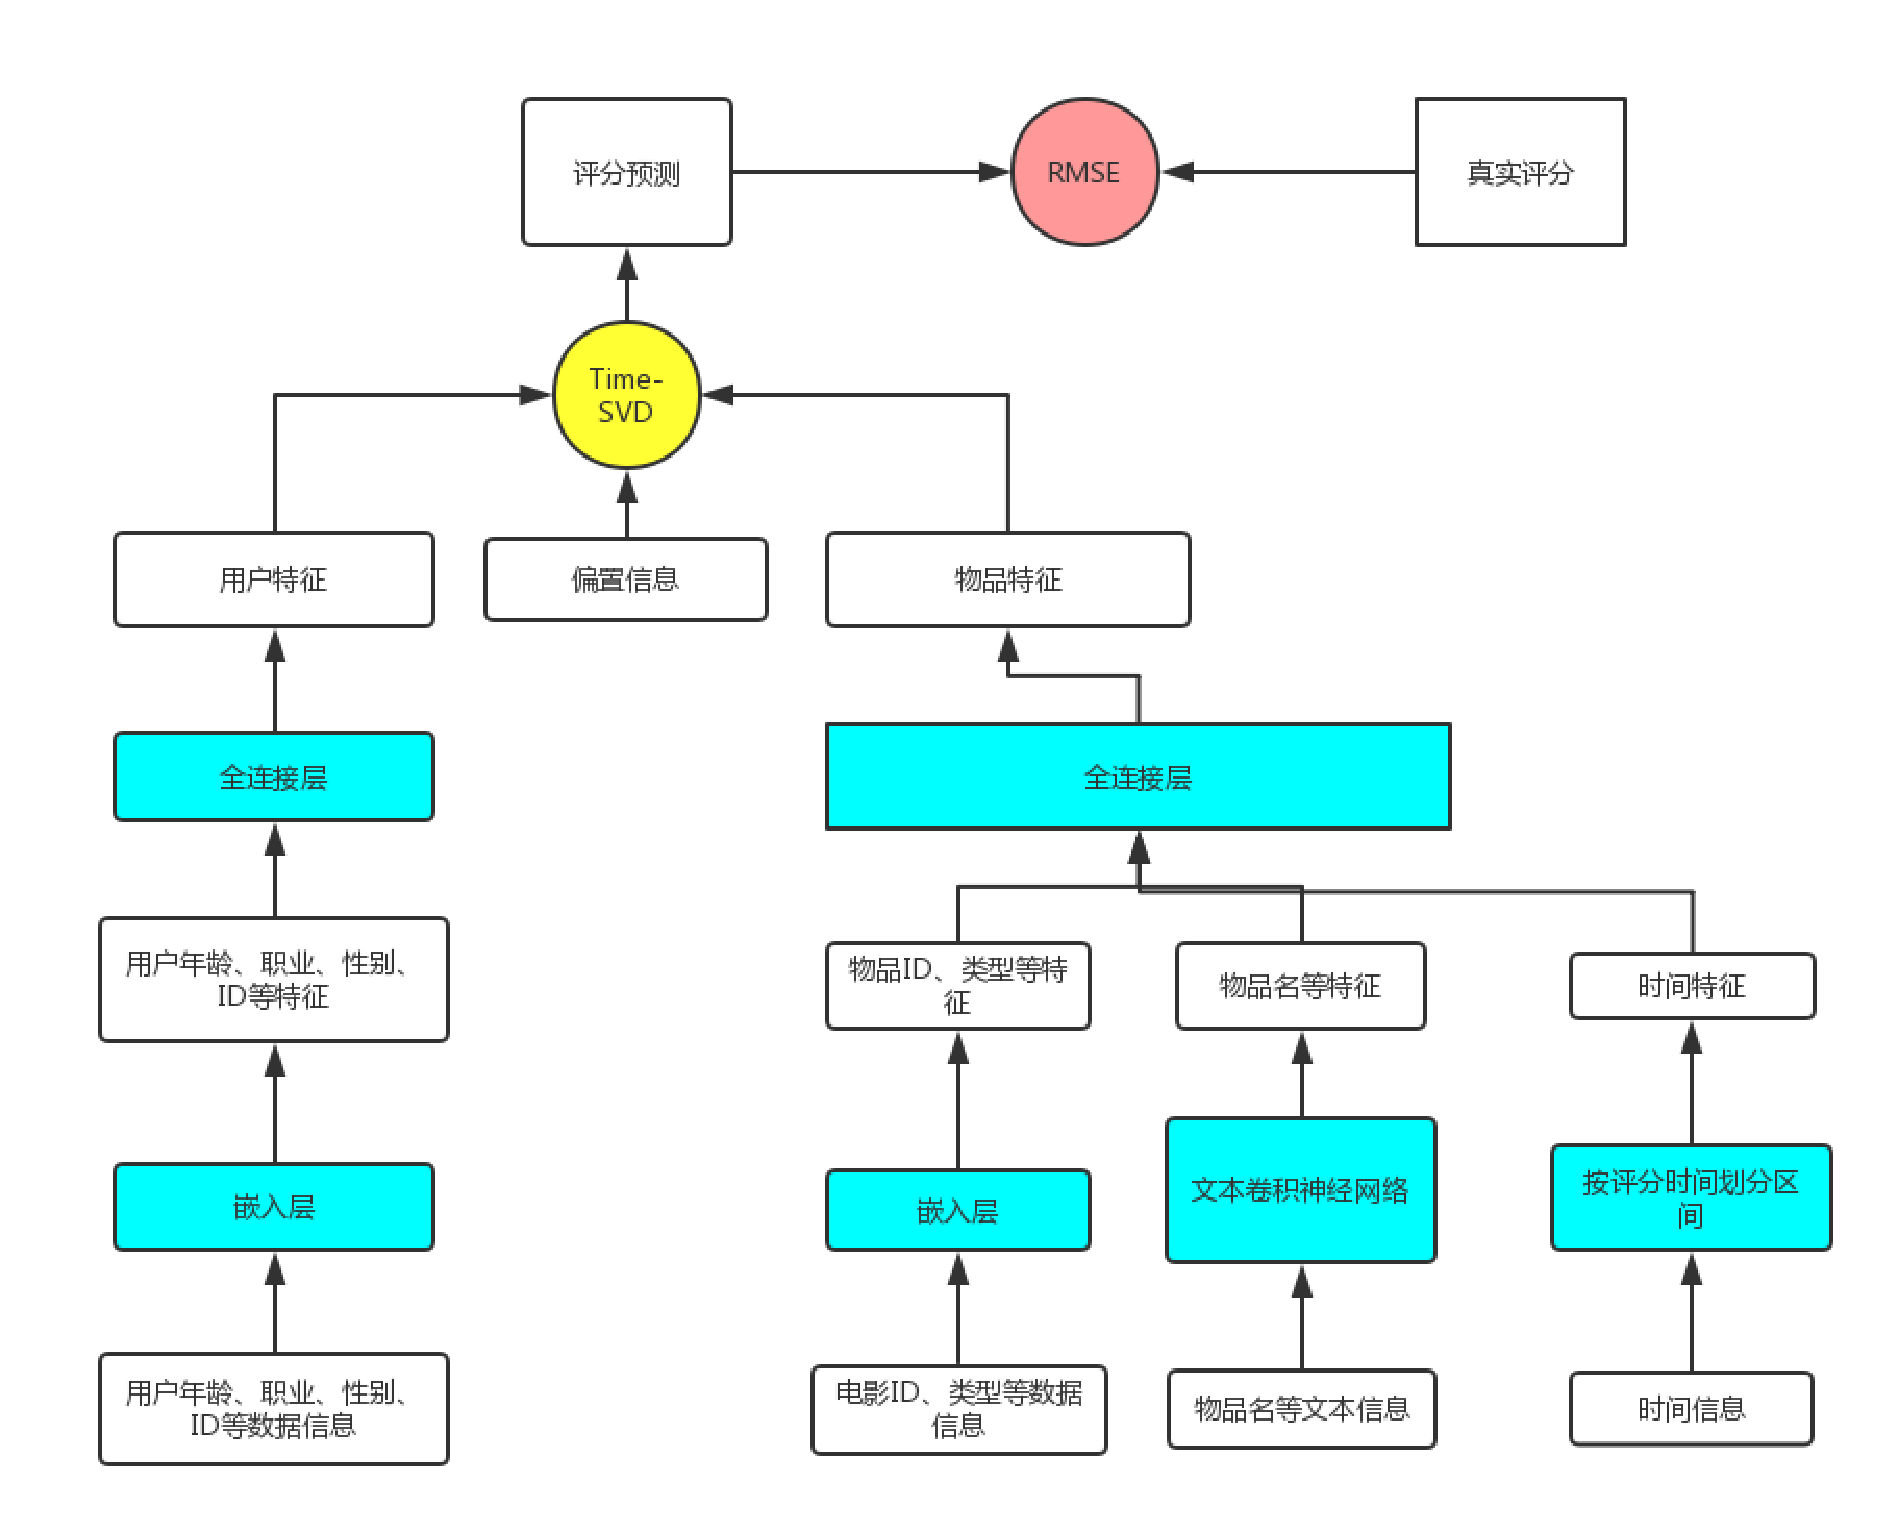
\includegraphics[width=0.8\linewidth]{images/myModel.pdf}
\caption{模型设计示意图}
\label{fig:fig1}
\end{figure}

基于上面所述内容,我们的研究将会在真实的数据集上,首先利用卷积神经网络将用户和物品中稀疏、高维的数据信息转化为稠密低维的特征信息。接下来再结合Time-SVD++的矩阵分解方法,将时间信息考虑进来,并与前面所得到的用户、物品向量一起建模,构建出一种如上图所示的,新型合理的评分预测模型。
\section{研究任务}
在这个背景下,我们的研究大致有如下几项任务:

1)获取并分析原始数据

本次实验我们主要使用MoviLens的1M数据集以及Netflix数据集。MovieLens数据集是由GroupLens通过收集整理电影评分网站MovieLens的评分数据而发布的,1M数据集包含6040个用户和3952部电影,共有1000209个用户评分记录。Netflix数据集则是由在线影片租赁商Netflix举办推荐竞赛时提供的。

2)数据预处理

原始的数据包含很多的类别字段,以电影类别为例就包含犯罪片、动作片、科幻片等不同的类型。为了更方便地处理数据,我们需要使用one-hot编码用数字来代替原始的类别字段。同时我们还需要对原始数据进行去去噪处理来提取关键项的数据。

3)使用卷积神经网络提取数据特征信息
用户部分的处理相对简单,我们需要将用户信息输入嵌入层,从嵌入层索引出特征以后,将特征传入全连接层,从而得到用户特征向量。而物品部分的处理则略有不同,这里我们需要额外使用文本卷积网络来单独处理物品名特征,之后再传入全连接层,与其他信息一起得到物品的特征向量。

4)矩阵分解建模

在建模部分我们借鉴了传统的Time-SVD++的方法,将评论的时间信息划分为不同的区间,利用不同的时间区间分别学习出隐因子向量,从而在建模时加入时间因素。同时我们还需要在建模阶段加入偏置信息,从而使得评分预测结果更具有普遍性。

5)实验和分析
在实验阶段我们需要评估模型在评分预测和top-N推荐方面的表现,并与常见的规范化矩阵奇异值分解(Funk-SVD)、非负矩阵分解(NMF)还有Time-SVD++方法进行比较。

评分预测中,我们使用均方根误差(root-mean-square error,RMSE)来评估预测的误差,其定义如下。

\begin{equation*}
RMSE = \sqrt{  \dfrac   {\sum\limits_{u,i \in T}  (r_{u,i} - \hat{r_{ui}}) ^2 } {|T|}   }.
\end{equation*}

对于测试集中的一个用户 $u$ 和物品 $i$ ,另 $r_{ui}$ 是用户 $u$ 对物品  $i$  的实际评分,而 $\hat{r_{ui}}$  是推荐算法给出的预测评分。

而在top-N推荐方面,我们则使用,命中率(Hit Ratio,HR)和归一化累积获得指标(Normalized Discounted Cumulative Gain,NDCG)来进行评估。

\chapter{技术路线}
\section{文本卷积神经网络(Text-CNN)}
卷积神经网络(CNN)在计算机视觉领域应用广泛,凭借其强大的局部特征捕捉能力,CNN为分析和利用图像数据的研究者提供了极大的帮助。而Yoon Kim等人\cite{Kim14fTextCNN}则将CNN应用到了文本分类中,提出了Text-CNN。在本研究中,Text-CNN被用来学习物品的文本信息,从而获得隐藏层向量。
TextCNN通常由四部分构成:输入层、卷积层、池化层、全连接层,如下图所示:

\begin{figure}[htbp]
\centering
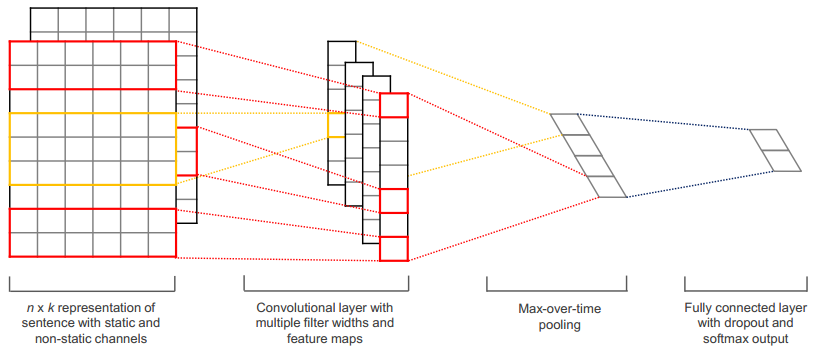
\includegraphics[width=0.8\linewidth]{images/textCNN.png}
\caption{TextCNN结构示意图}
\label{fig:fig2}
\end{figure}



1)输入层

输入层是句子中词向量自上而下排列的矩阵,假如句子中有$n$个词,向量的维数是$k$,那么输入层就是一个$n\times k$的矩阵。
这里,我们用$x_i \in  \mathbb{R}^k$来表示句子中第$i$个$k$维向量。那么一个长度为$n$的句子就可以表示为:

\begin{equation}
x_{1:n} = x_1 \oplus x_2 \oplus ...\oplus x_n
\end{equation}
2)卷积层

在卷积层需要做的一件事就是卷积。卷积操作常用来做图像处理,就是取一定窗口大小的图像矩阵与滤波器(权重矩阵)做内积(逐个元素相乘再相加)。
用数学公式表示就是,用$w \in \mathbb{R}^{hk}$来表示滤波器,那么一个特征$c_i$就是由一个窗口中的词语$x_{i:i+h-1}$所生成:
\begin{equation}
c_i = f(w\cdot x_{i:i+h-1} + b)
\end{equation}
这里$b\in \mathbb{R}$是偏置项,而$f$则是像双曲函数这样的非线性函数。
这里,我们就可以从句子里每$h \times k$的窗口${x_1:h,x_2:h,...,x_{n-h+1:n}}$通过卷积操作得到若干个特征图(Feature Map)
\begin{equation}
c = [c_1, c_2,...,c_{n-h+1}]
\end{equation}

其中$c \in \mathbb{R}^{n-h+1}$

3)池化层

在池化层中,TextCNN采用了一种称为Max-over-time Pooling的方法。该方法从之前得到的一维特征图中提取出最大值:$\hat{c} = \max\{c\}$。因为最大值往往代表着最重要的信号。而同时,因为不管特征图中有多少值,只需提取出其中的最大值,池化操作也可以解决不同长度的句子输入问题。
最终池化层输出的结果为各个特征图的最大值的集合,即一个一维向量。

4)全连接层

在TextCNN中,池化层中的一维向量的输出通过全连接的方式连接到Softmax层中进行分类。而在全连接层中则使用Dropout技术,并对全连接层上的权重参数给予L2正则化的限制,从而防止过拟合的发生。
举例来说,如果我们用$m$来表示滤波器的个数,那么池化层的输出结果就可以用$z = [\hat{c_1},...,\hat{c_m}]$来表示。在正则化阶段,dropout会使用如下方式来优化权重参数$w$
\begin{equation}
y = w\cdot(z \circ r) + b
\end{equation}
这里$\circ$ 是向量按位乘法的操作,而$r\in \mathbb{R}^m$则是由概率值$p$为1的伯努利随机变量所生成的屏蔽向量(masking vector)。

\section{奇异值分解(SVD}

\subsection{基本的奇异值分解}
奇异值分解(SVD)是一种最基本的矩阵分解方式,它的核心思想是认为用户的兴趣只受少数几个因素$k$的影响,因此将稀疏且高维的User-Item评分矩阵分解为两个低维矩阵,如下所示。
\begin{equation}
U_{m\times k}V_{n\times k}^T \approx A_{m \times n}
\end{equation}
这里$m$代表用户数量,$n$代表物品数量,$k$代表选取的特征数量。真实数据集中$m$和$n$的值很大,而$k$相比之下要小很多,至少两个数量级以上。
而要计算物品$i$推荐给用户$u$的推荐分数,则需要计算内积,如下所示。
\begin{equation}
\hat{r_{ui}} = q_i^Tp_u
\end{equation}
其中$p_u$和$q_i$分别为用户$u$和物品$i$的特征向量。
但是大多数真实数据集上的评分矩阵都是相当稀疏的,所以它只关注这些很少的值会导致过拟合问题。早期通过填补矩阵中缺失的评级使矩阵变得稠密,但是随着可见项的增加,计算量可能难以承受,另外,不准确的填充会严重影响预测的效果。可以通过引入正则项缓解过拟合的问题,为了得到特征向量,系统最小化在已知评分上的正则平方误差:
\begin{equation}
\min_{q^*, p^*} {\sum\limits_{(u,i) \in \kappa} {{(r_{u,i}-q_i^Tp_u)}^2 + \lambda(||q_i||^2 + ||p_u||^2)} } ,
\end{equation}
这里,$\kappa$ 是训练集中所有已知评级的用户物品对 $(u,i)$ 的集合,系统通过拟合之前观测的样本来学习模型的参数,而我们的目标是预测未知的评分,所以应该通过正则化参数来避免过度拟合已知的项,常数 $\lambda$ 用于控制正则化的程度。可以通过随机梯度下降或迭代最小二乘的方法最小化上面的式子。


\subsection{带偏置的奇异值分解}

基本的矩阵分解方法通过学习用户和物品的特征向量进行预测,其中用户的特征向量代表了用户的兴趣,物品的特征向量代表了物品的特点。但是我们观测到的评分数据中,有很大一部分与用户对物品的喜好无关而只取决于用户或物品本身的特性。以电影推荐为例,标准宽松的用户往往会给出偏高的评分,而相对严格的用户的评分则普遍偏低;而同样,受大众欢迎的电影,往往会得到偏高的评分,而一些烂片的评分则普遍偏低。
我们把独立于用户或物品的因素称为偏置(Bias)部分,可以用如下公式来表示。
\begin{equation*}
b_{ui} = \mu + b_u + b_i
\end{equation*}

$\mu$是训练集中所有评分记录的全局平均数,它表示了训练数据的总体评分情况。$b_u$是用户偏置,表示某一特定用户的打分习惯。$b_i$是物品偏置,表示某一特定物品得到的打分情况。
接下来进行参数优化,损失函数如下所示:
\begin{equation}
\min_{q^*, p^*} {\sum\limits_{(u,i) \in \kappa} {{(r_{u,i}-\mu-b_u-b_i-q_i^Tp_u)}^2 + \lambda(||q_i||^2 + ||p_u||^2 + b_u^2 + b_i^2)} } ,
\end{equation}
其中参数$q_i$、$p_u$、$b_u$、$b_i$仍然可以采用交替最小二乘或随机梯度下降进行优化。
而加入以上偏置信息的评分预测公式如下所示。
\begin{equation}
\hat{r_{ui}} = \mu + b_u + b_i + q_i^Tp_u
\end{equation}

\subsection{加入时间动态的奇异值分解}
在上面加入偏置信息的基础上,我们仍然需要考虑两个变化性的因素:一方面,每个物品的受欢迎程度$b_i$会随着时间变化而变化;另一方面,用户的评价标准$b_u$也会随时间而发生改变,我们使用如下公式来表示。
\begin{equation}
b_{ui}(t) = \mu + b_u(t) + b_i(t)
\end{equation}
这里$b_{ui}(t)$表明第$t$天用户$u$对物品$i$的基准评价,而$b_u(t)$和$b_i(t)$则是用户和物品偏置随着时间而改变的具体函数值。
这里我们需要对时间按区间划分为时间段,每个时间段内使用一个不同的值。

对于物品来说:
\begin{equation}
b_i(t) = b_i + b_{i,Bin(t)}
\end{equation}
其中$Bin(t)$为时间对应的函数。

而对于用户$u$,我们用$t_u$表示时间的平均值,那么用户打分对于时间$t$的导数$dev_u(t)$可以表示为:

\begin{equation*}
dev_u(t) = sign(t - t_u)\cdot |t - t_u|^\beta
\end{equation*}
这里的$|t - t_u|$是用来衡量时间$t$和$t_u$之间的距离。
于是用户偏好关于时间的偏置信息可以表示为:
\begin{equation}
b_u(t) = b_u + \alpha_u \cdot dev_u(t)
\end{equation}
新的损失函数为:
\begin{equation*}
\min_{u, i, t} {\sum\limits_{(u,i) \in \kappa} {{(r_{u,i}(t)-\mu-b_u - \alpha_udev_u(t)-b_{u,t}-b_i - b_{i,Bin(t)}}^2 + \lambda(b_u^2 + \alpha_u^2 + b_{u,t}^2 + b_i^2 + b_{i,Bin(t)}^2))}} 
\end{equation*}

于是我们得到了将用在本次研究的评分预测公式:
\begin{equation*}
\hat{r_{ui}} = \mu + b_u(t) + b_i(t) + q_i^Tp_u(t)
\end{equation*}
\chapter{可行性分析}
1)数据可行性

互联网的飞速发展在改变人们生活方式的同时,也将用户的行为数据保存了下来。不管是用户显示的打分数据,还是点击、浏览商品时产生的隐式反馈数据,这其中都蕴含着丰富的潜在信息,来等待商家还有研究者进行挖掘。而这也为推荐系统领域的相关研究带来了广泛而多样的数据集。

以我们本次所将使用的MovieLens数据集为例,其中就包含用户数据users.dat,电影数据movies.dat还有评分数据ratings.dat。其中的用户数据包含用户ID、性别、年龄、职业和邮编等,这些数据可以在研究中用来学习用户的特征向量,电影数据中的ID、风格则可以用来学习物品的特征向量,其中的电影名作为文本信息则可以利用TextCNN来进行处理。而评分数据中的时间戳字段则可以用来发现用户的兴趣漂移规律,其中的评分数据则可以分成训练集和测试集,分别用来优化参数和评估模型的实际效果。

2)环境可行性

当前推荐系统的研究依然火热,从最早的Netflix电影推荐大赛,KDD Cup数据挖掘竞赛,再到前段时间的阿里移动推荐大赛,京东的JData算法大赛。用于改进推荐算法的竞赛层出不穷,各家平台甚至拿出不菲的奖金来鼓励参赛者对自己现有的推荐算法进行改进。由此可见,在当前外部环境研究推荐算法的改进策略是顺势而为,大势所趋。

3)技术可行性

虽然在推荐系统领域,深度学习还处于一个新兴的阶段。但其在文本处理等方面的成功应用,也为其在挖掘用户和物品的关联信息等方面提供了借鉴。而谷歌推出的TensorFlow,Facebook推出的pytorch,当下也已经成为应用非常广泛的深度学习框架,方便研究者进行深度学习方面的研究。而前面提到的Time-SVD++和TextCNN技术都已经在相应数据集上跑出了不错的效果,其学习过程均可收敛从而达到最优解。由此可见,本次基于深度学习的矩阵分解算法研究具有较高的技术可行性。

4)经济可行性

我们本次使用的均是平台上公开的真实数据集,且仅用于研究,而非处于商业目的。且研究过程主要依赖软件来实现,同时实验所在的浙大电子服务研究中心也已经配备了装有Tesla K40c GPU的服务器,可以用于加速接下来深度学习实验的进行。
\chapter{预期目标及研究计划进度安排}

\section{预期目标}

本次的推荐算法研究,旨在利用卷积神经网络来挖掘数据中的隐含关联信息,并结合矩阵分解,融合时间信息因素,提出一种合理的推荐算法模型,并希望能在RMSE等评分预测指标以及HT、NDCG等衡量top-N推荐质量的指标上,相比于传统的矩阵分解模型有一定程度的改进,缓解推荐时常遇到的数据稀疏和冷启动问题。
\section{进度安排} 
根据之前所述的研究方法和预期结果,将论文的进度计划安排如下:

\begin{table}[h]
\centering
\label{my-label}
\begin{tabular}{cc}
\hline
\rowcolor[HTML]{EFEFEF} 
\textbf{时间}           & \textbf{进度安排}                \\ \hline
2017.7 - 2017.12      & 阅读相关文献资料,充分理解现有的研究成果,并撰写文献综述 \\ \hline
2018.3.1 - 2018.3.20  & 提出初步的研究方案,与导师进行讨论,做出补充和改进    \\ \hline
2018.3.21 - 2018.4.1  & 根据研究方案确定初步的模型,并撰写开题报告                \\ \hline
2018.4.2 - 2018.4.10 & 获取实验数据,分析数据并进行预处理            \\ \hline
2018.4.11 - 2018.4.25 & 实现论文中的关键算法,并在数据集上测试效果        \\ \hline
2018.4.26 - 2018.5.5 & 对比不同算法,并对各项指标进行分析            \\ \hline
2018.5.6 - 2018.5.15 & 对研究结果进行归纳,整理实验数据,完成论文初稿      \\ \hline
2018.5.15 - 2018.5.30  & 完善和修改,并确定论文终稿                \\ \hline
\end{tabular}
\end{table}



\bibliography{data/kaiti}







